\documentclass[10pt]{beamer}

\mode<presentation> {

\usetheme{Madrid}  % Circles & dense

\setbeamertemplate{headline}{%
\leavevmode%
  \hbox{%
    \begin{beamercolorbox}[wd=\paperwidth,ht=2.5ex,dp=1.125ex]{palette quaternary}%
    \insertsectionnavigationhorizontal{\paperwidth}{}{\hskip0pt plus1filll}
    \end{beamercolorbox}%
  }
}

\setbeamertemplate{navigation symbols}{}

}

\setbeamertemplate{caption}[numbered]

\usepackage{graphicx}
\usepackage{booktabs}
\usepackage{fontspec}
\usepackage{amsmath}
\mathchardef\mhyphen="2D % Define a "math hyphen"
\usepackage{caption}
\usepackage{xunicode}
\usepackage{xltxtra}
\usepackage{lipsum}
\usepackage{xecyr}
\usepackage{hyperref}
\usepackage{amsthm}
\usepackage{blindtext}
\usepackage{makecell}
\usepackage{multirow}
\usepackage{array}
\usepackage{siunitx}
\usepackage{booktabs}
\usepackage{bigdelim}
\usepackage{multicol}

\usepackage{polyglossia}
\setdefaultlanguage{english}
\setotherlanguages{russian}
\setmainfont[Mapping=tex-text]{CMU Serif}
\setsansfont[Mapping=tex-text]{CMU Sans Serif}
\setmonofont[Mapping=tex-text]{CMU Serif}

\newread\tmp
\openin\tmp=main.bib%
\read\tmp to \bib%
\closein\tmp%
\begin{filecontents}[overwrite]{\jobname.bib}
\bib
\end{filecontents}
\usepackage[style=verbose,backend=biber]{biblatex}
\addbibresource{main.bib}

\definecolor{green}{RGB}{0, 200, 0}

\addto\captionsenglish{%
  \renewcommand{\figurename}{Фигура}%
  \renewcommand{\tablename}{Таблица}%
}

% Title
\title[Speech Synthesis]{TalkNet: Fully-Convolutional Non-Autoregressive Speech Synthesis Model}
\author[Stanislav Beliaev]{Stanislav Beliaev, Boris Ginsburg}
\institute[NVIDIA]{NVIDIA}
\date{05/26/2020}

\begin{document}

\begin{frame}
\titlepage
\end{frame}

\section{Introduction}

\begin{frame}
\begin{block}{Speech Synthesis}
Generate audio sample from input text sequence.
\end{block}
There are two parts in pipeline usually: generating mel-spectrogram and vocoding.
\begin{figure}[H]
\centering
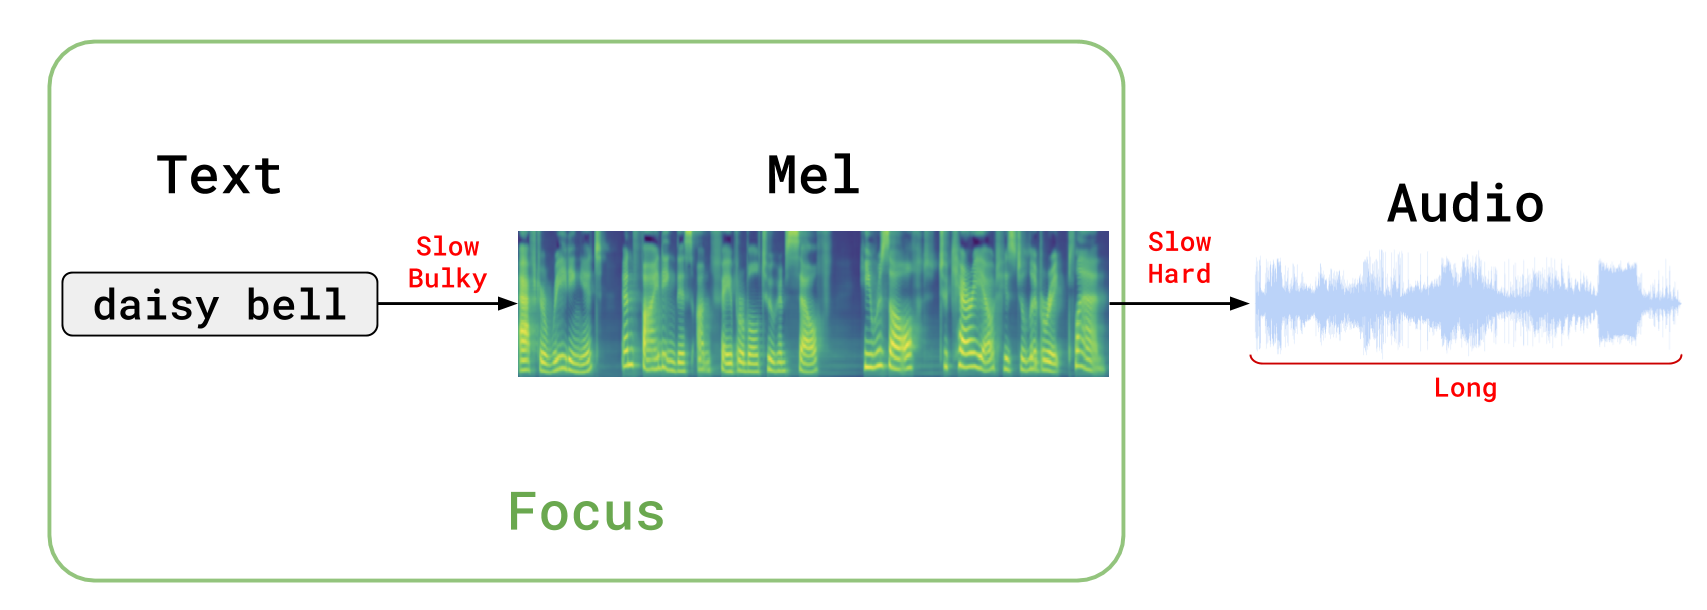
\includegraphics[width=1.0\textwidth]{images/tts-pipeline.png}
\end{figure}
\end{frame}

\begin{frame}
\begin{itemize}
    \item Tacotron2~\footcite{tacotron2}: 30M weights, slow autoregressive inference (RNN), robustness problem, good quality.
    \item Transformer-TTS~\footcite{transformer-tts}: 60M weights, slow autoregressive inference, robustness problem, a bit better quality.
    \item FastSpeech~\footcite{fastspeech}: 30M weights, requires another pretrained attention-based TTS model as teacher, fast and comparable quality.
\end{itemize}
\end{frame}

\begin{frame}{Non-autoregressive approach}
\begin{figure}[H]
\centering
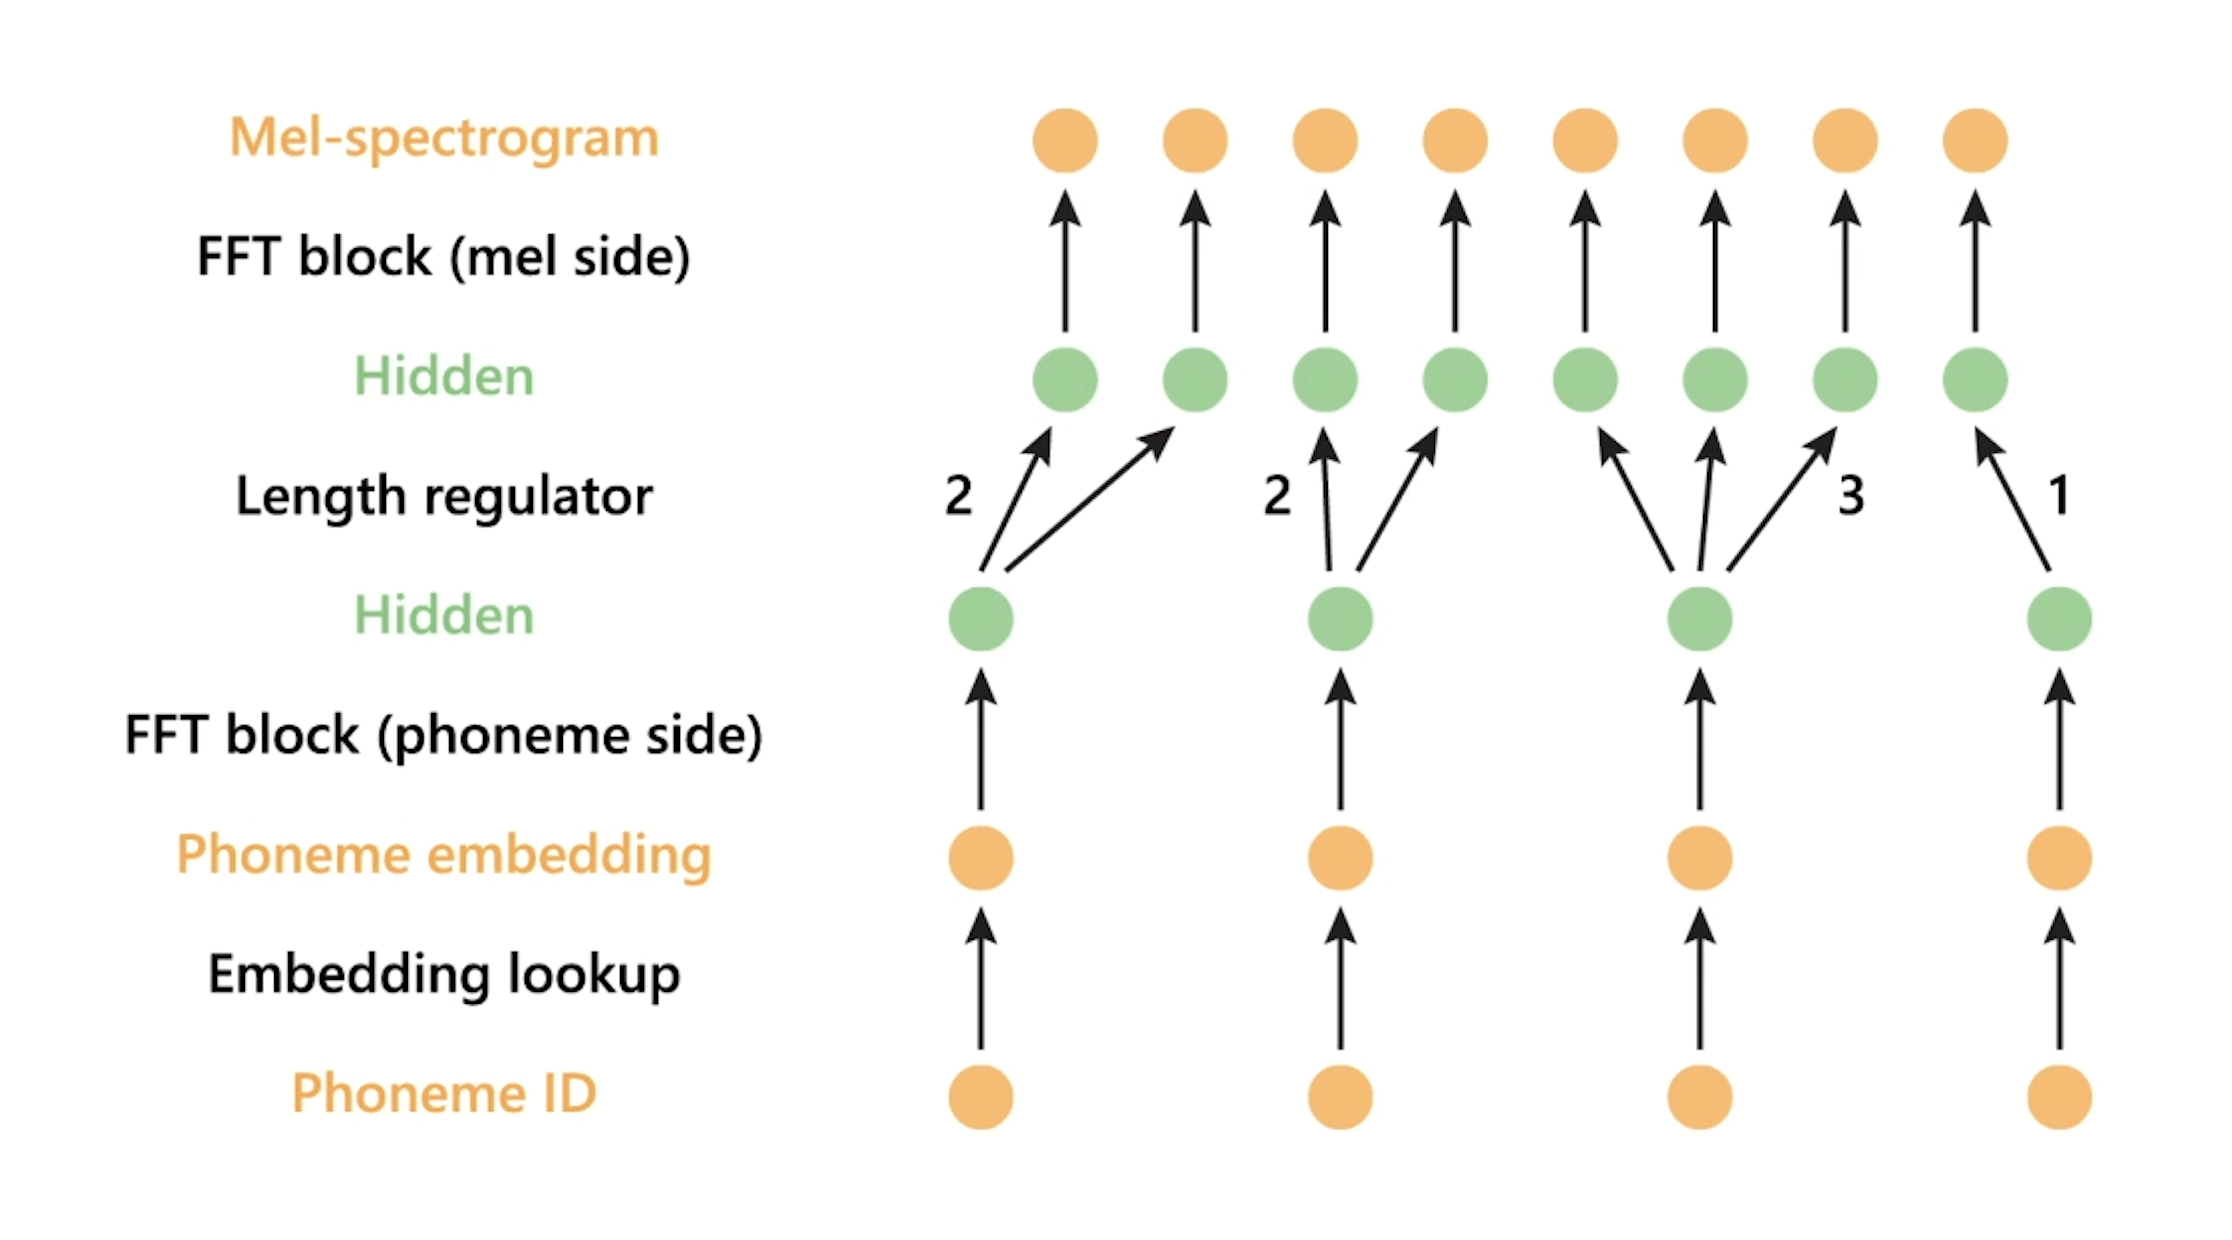
\includegraphics[width=1.0\textwidth]{images/fastspeech/alignment.png}
\end{figure}
\end{frame}

\begin{frame}{FastSpeech}
\begin{figure}[H]
\centering
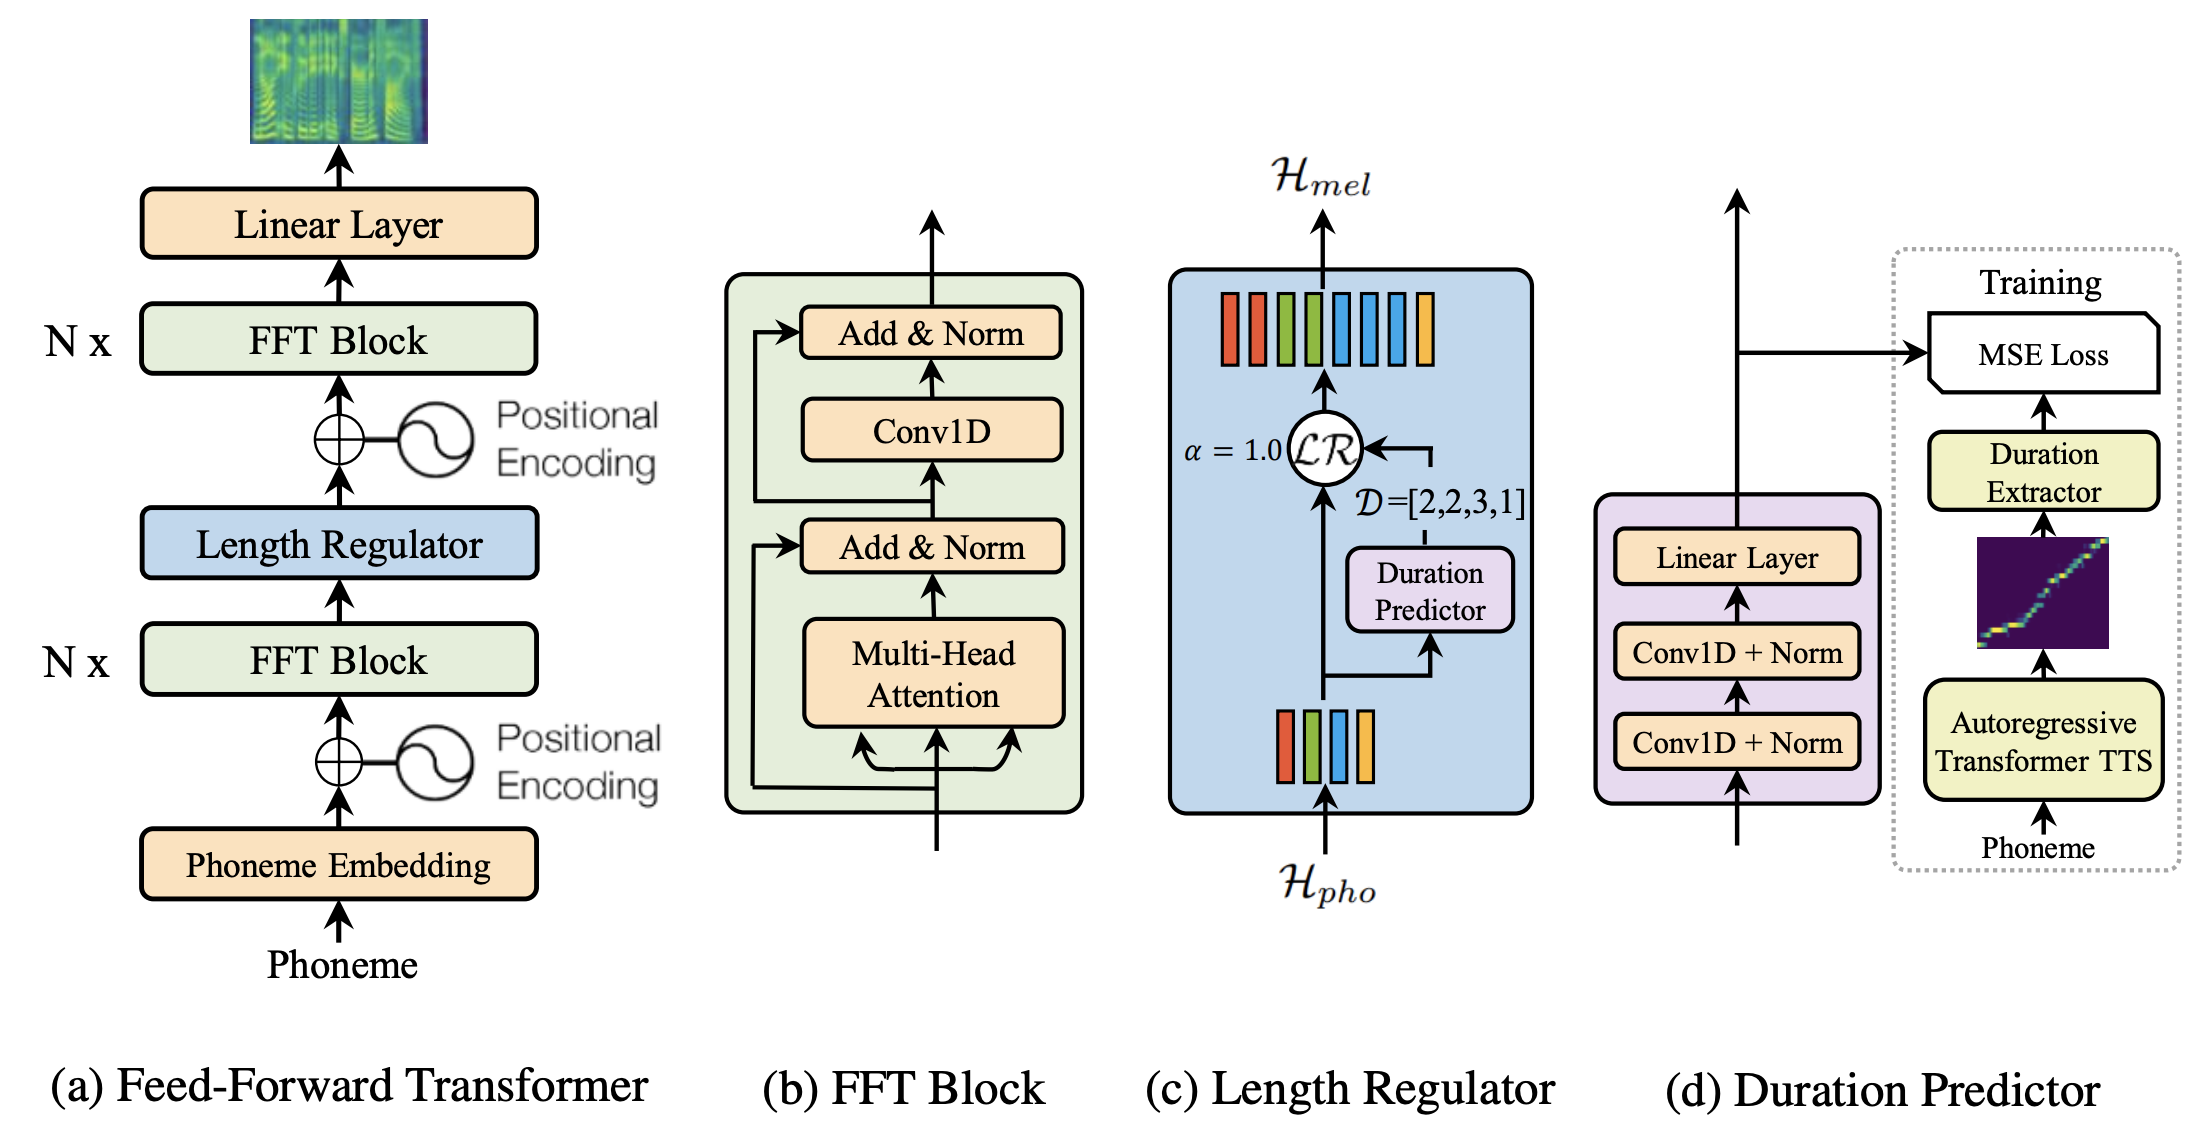
\includegraphics[width=1.0\textwidth]{images/related-work/fastspeech.png}
\end{figure}
\end{frame}

\begin{frame}
Our \underline{goal} was to develop lightweight and fast speech synthesis models maintaining comparable quality and robustness.

\underline{Tasks}:
\begin{itemize}
    \item Analyze competitors.
    \item Describe architecture.
    \item Make experiments.
    \item Analyze quality and speed.
\end{itemize}
\end{frame}

\section{Architecture}

\begin{frame}{Idea}
\begin{itemize}
    \item We split generation pipeline into two separate stages: graphemes durations prediction and mel-spectrogram generation.
    \item We build a way to extract GT durations from pretrained ASR model.
    \item Both nets are fully-convolutional non-autoregressive NNs.
\end{itemize}
\end{frame}

\begin{frame}
\begin{figure}[H]
\centering
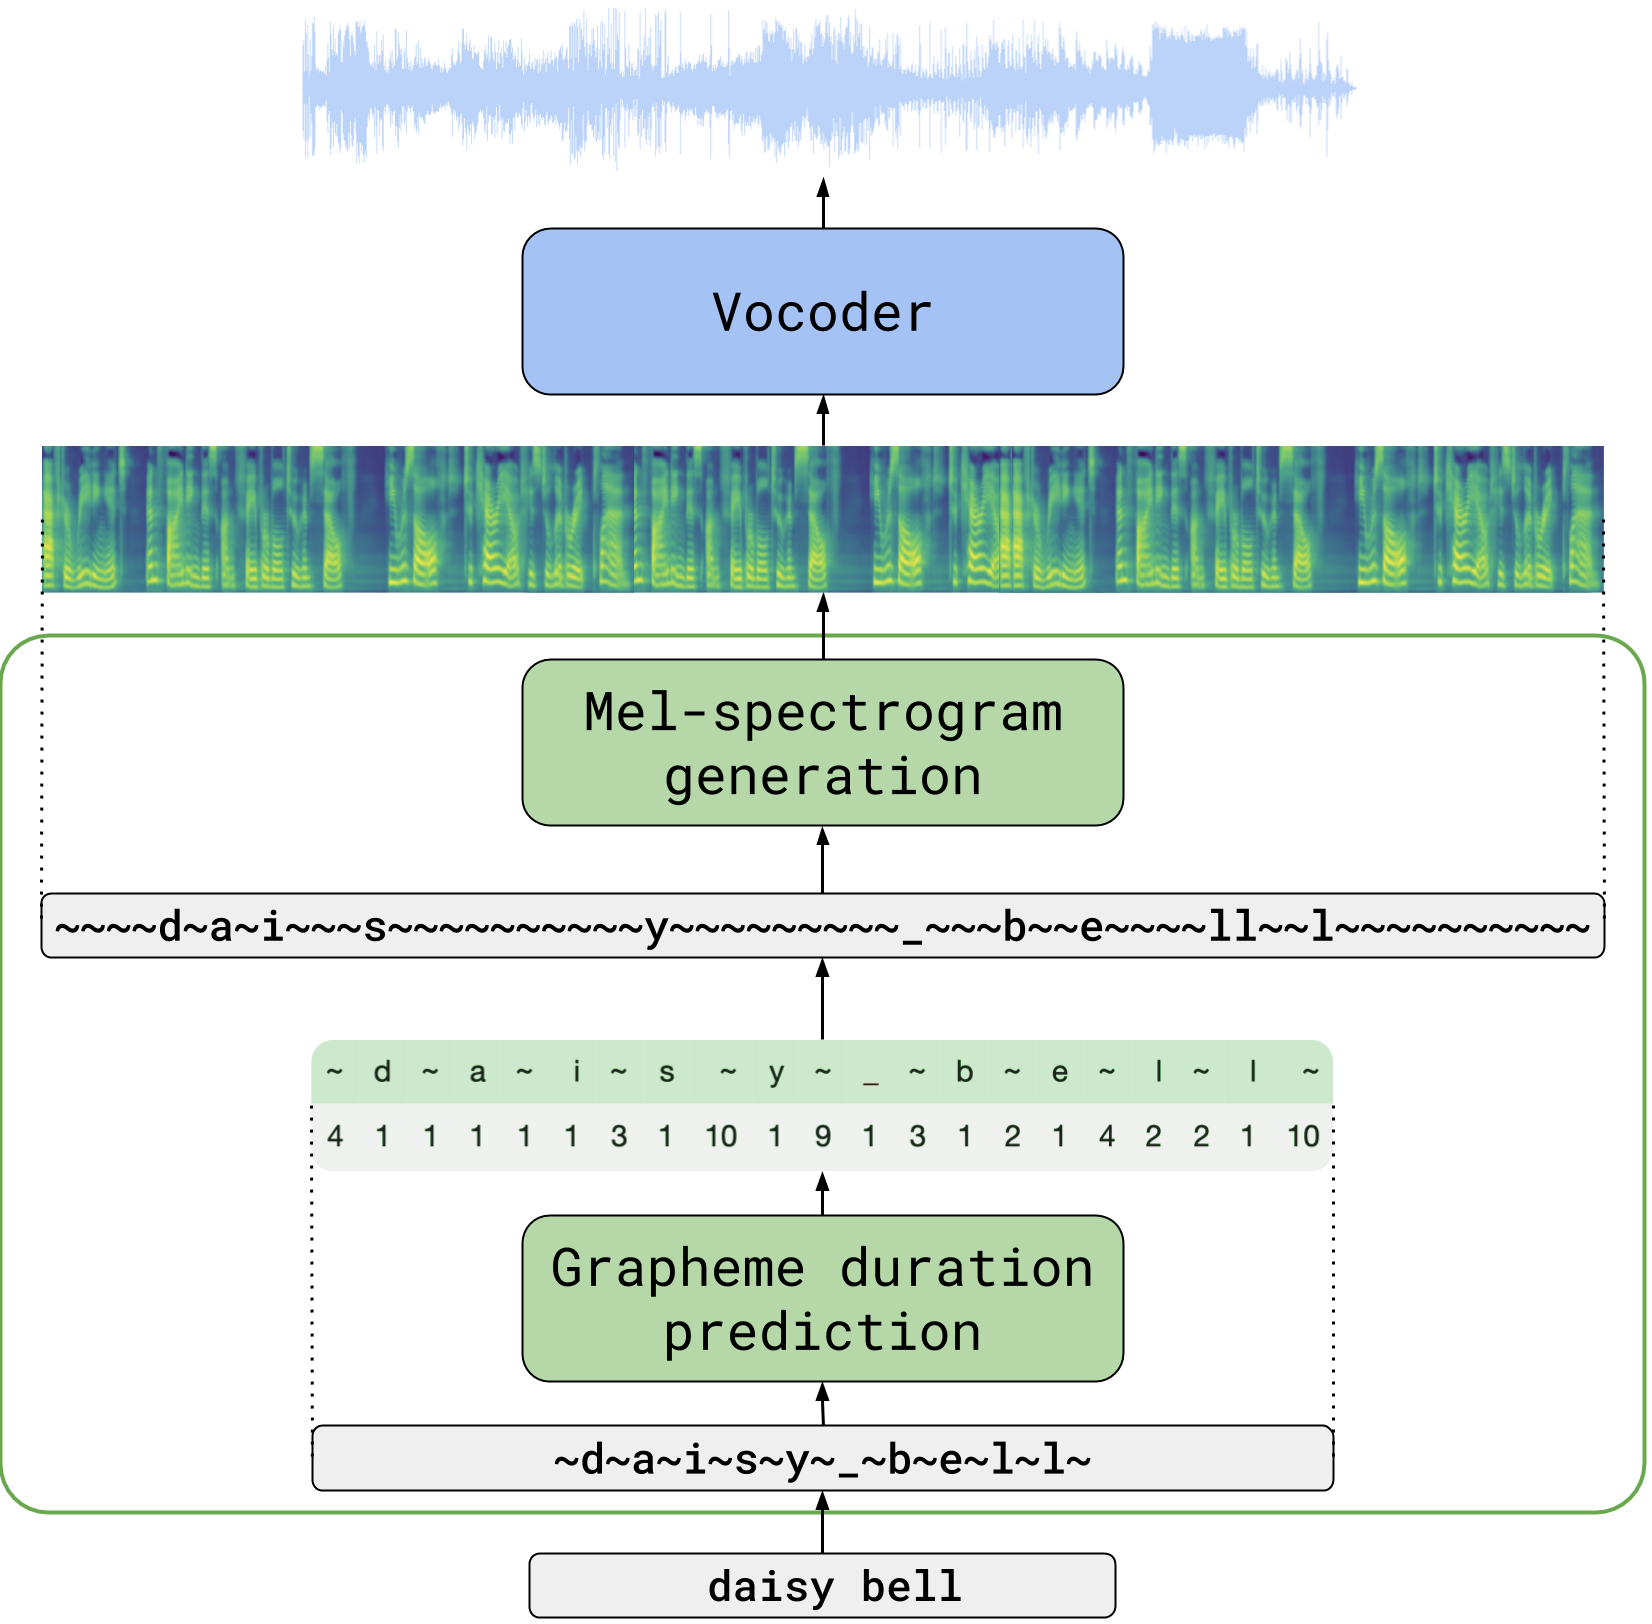
\includegraphics[width=0.7\textwidth]{images/arch.png}
\end{figure}
\end{frame}

\begin{frame}
\begin{figure}[H]
\centering
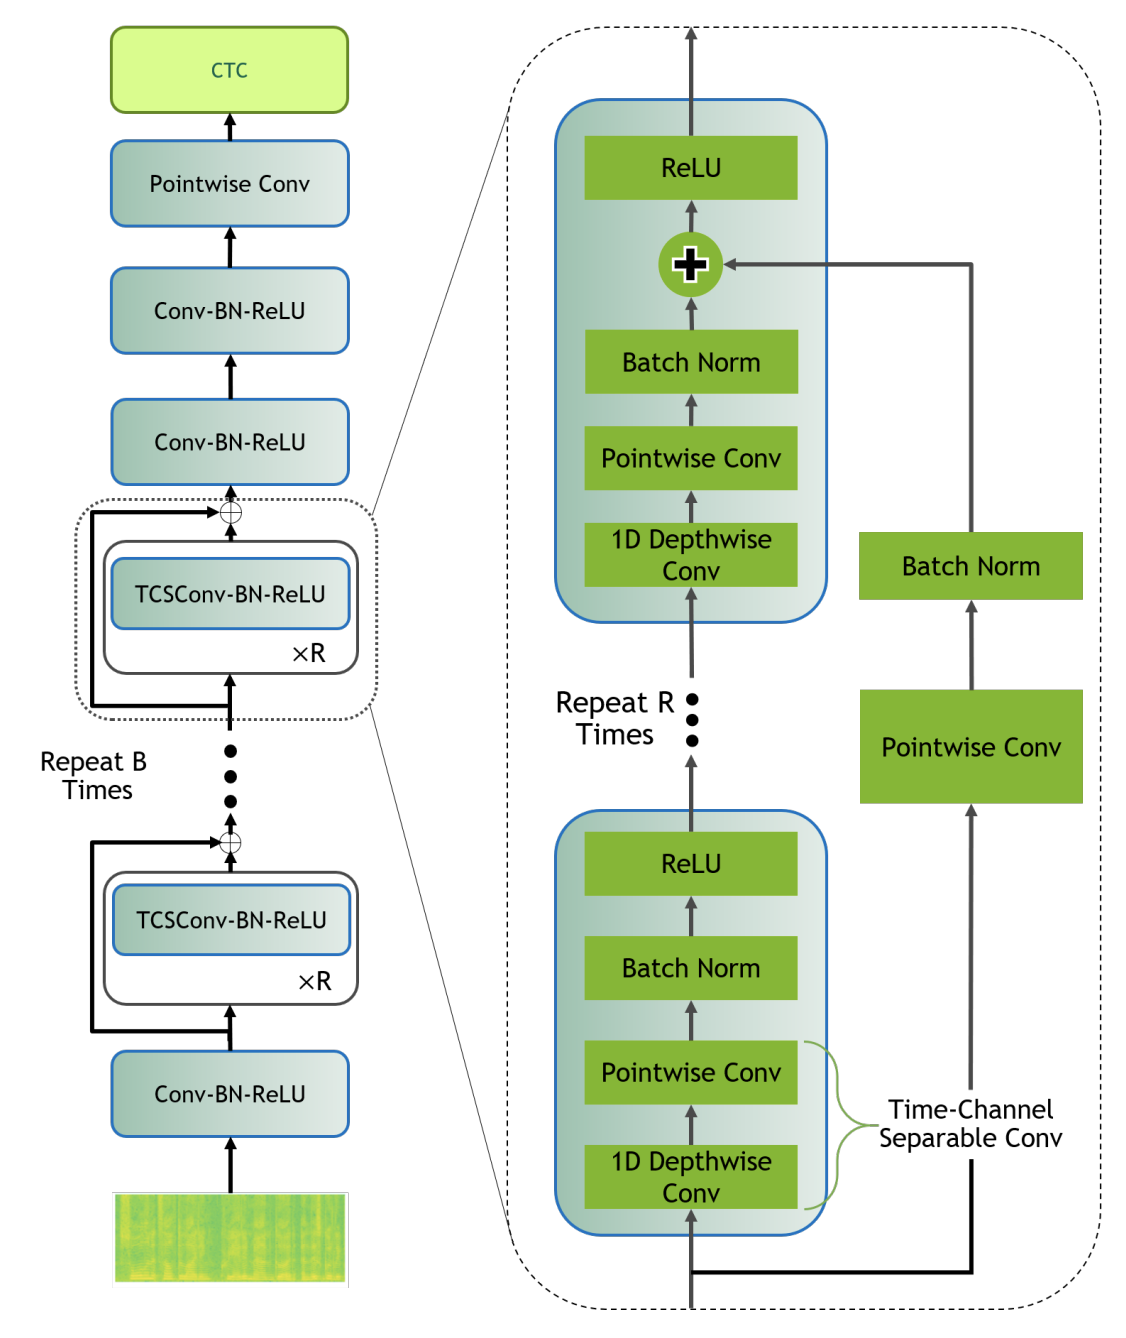
\includegraphics[width=0.5\textwidth]{images/qn.png}
\caption{QuartzNet~\footcite{quartznet} solves reverse task: speech recognition. CTC learns time alignment between mel and text.}
\end{figure}
\end{frame}

\begin{frame}
\begin{figure}[H]
\centering
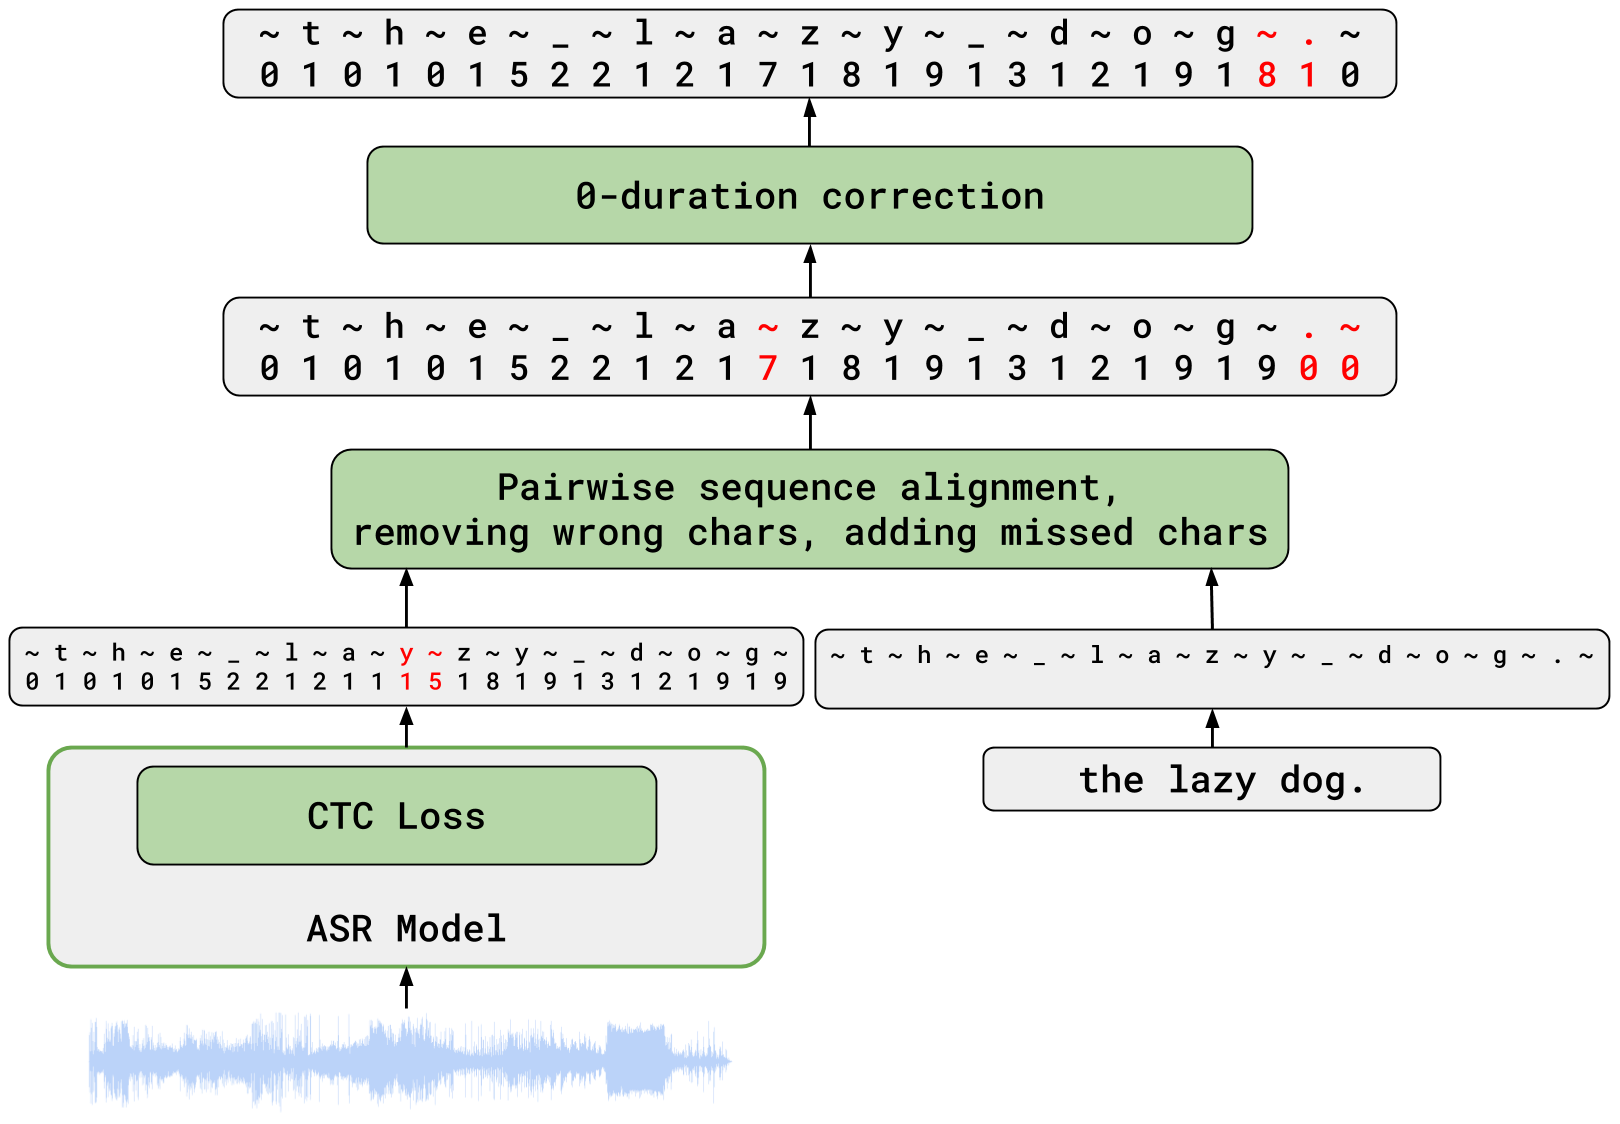
\includegraphics[width=1.0\textwidth]{images/alignment.png}
\end{figure}
\end{frame}

\section{Training}

\begin{frame}{Training}
\begin{itemize}
    \item Both nets were based on QuartzNet architecture.
    \item Whole pipeline takes just around 2 hours to converge on DGX-1.
    \item We design a way to augment GT durations in an unbiased way to introduce robustness with respect to changes.
\end{itemize}
\end{frame}

\begin{frame}
\begin{table}[ht!]
\centering
\scalebox{0.85}{
\begin{tabular}{c c c c c} 
\toprule
\textbf{Block} &
\textbf{\thead{\# Sub\\Blocks}} &
\textbf{\thead{\# Output\\Channels}} &
\textbf{Kernel Size} &
\textbf{Dropout} \\
\midrule
Embed & 1 & 64  & 1 & 0.0  \\
Conv1 & 3 & 256 & 3 & 0.1  \\
$B_1$ & 5 & 256 & 5 & 0.1  \\
$B_2$ & 5 & 256 & 7 & 0.1  \\
$B_3$ & 5 & 256 & 9 & 0.1  \\
$B_4$ & 5 & 256 & 11 & 0.1 \\
$B_5$ & 5 & 256 & 13 & 0.1 \\
Conv2 & 1 & 512 & 1 & 0.1  \\
Conv3 & 1 & $32$ & 1 & 0.0 \\
\midrule
\textbf{Parameters (millions)} & & & & \textbf{2.3} \\
\bottomrule
\end{tabular}
}
\caption{Grapheme duration predictor based on QuartzNet 5x5. It takes just around 15 minutes for net to converge on LJSpeech data on DGX-1.}
\end{table}
\end{frame}

\begin{frame}
\begin{table}[!ht]
\centering
\scalebox{1.0}{
\begin{tabular}{c c c c c} 
\toprule
\textbf{Block} &
\textbf{\thead{\# Sub\\Blocks}} &
\textbf{\thead{\# Output\\Channels}} &
\textbf{Kernel Size} &
\textbf{Dropout} \\
\midrule
Embed & 1 & 256 & 1 & 0.0 \\
Conv1 & 3 & 256 & 3 & 0.0 \\
$B_1$ & 5 & 256 & 5 & 0.0 \\
$B_2$ & 5 & 256 & 7 & 0.0 \\
$B_3$ & 5 & 256 & 9 & 0.0 \\
$B_4$ & 5 & 256 & 13 & 0.0 \\
$B_5$ & 5 & 256 & 15 & 0.0 \\
$B_6$ & 5 & 256 & 17 & 0.0 \\
$B_7$ & 5 & 512 & 21 & 0.0 \\
$B_8$ & 5 & 512 & 23 & 0.0 \\
$B_9$ & 5 & 512 & 25 & 0.0 \\
Conv2 & 1 & 1024 & 1 & 0.0 \\
Conv3 & 1 & 80 & 1 & 0.0 \\
\midrule
\textbf{Params, M} & & & & \textbf{8.5} \\
\bottomrule
\end{tabular}
}
\caption{Mel-spectrogram generator is based on QuartzNet~9x5. It takes just around 2 hours for net to converge on LJSpeech data on DGX-1.}
\end{table}
\end{frame}

\section{Results}

\begin{frame}
\begin{table}[!ht]
\centering
\scalebox{1.0}{
\begin{tabular}{l c} 
\toprule
\textbf{Model} &
\textbf{MOS} \\
\midrule
Ground truth speech & $4.31 \pm 0.05$ \\
Ground truth mel + WaveGlow & $4.04 \pm 0.05$ \\
Tacotron 2 + WaveGlow & $3.85 \pm 0.06$ \\
% FastSpeech~\cite{Fastspeech2019} & $\star \pm \star$ \\
\midrule
TalkNet + WaveGlow & $3.74 \pm 0.07$ \\
\bottomrule
\end{tabular}
}
\caption{MOS scores with $95\%$ confidence interval. We used NVIDIA's implementation for Tacotron 2 and WaveGlow. We tested $100$ audio samples with $10$ people per sample. The scores ranged from $1.0$ to $5.0$ with a step of $0.5$.}
\end{table}
\end{frame}

\begin{frame}
\begin{table}[!ht]
\centering
\scalebox{1.0}{
\begin{tabular}{l l l r} 
\toprule
\textbf{Model} & 
\textbf{Batch} &
\textbf{Latency, s} &
\textbf{RTF} \\
\midrule
Transformer TTS & 1 & $6.735 \pm 3.969$ & $1.48 \pm 0.87$ \\
Tacotron 2 & 1 & $0.817 \pm 1\cdot 10^{-2} $ & $7.56 \pm 0.01$ \\
FastSpeech & 1 & $0.029 \pm 2 \cdot {10}^{-4}$ & $221.01 \pm 1.75$ \\
\midrule
TalkNet & 1 & $0.019 \pm 1 \cdot {10}^{-5}$ & $328.65 \pm 4.76$ \\
TalkNet & 4 & $0.023 \pm 5 \cdot {10}^{-5}$ & $1048.80 \pm 21.75$ \\
TalkNet & 8 & $0.037 \pm 4 \cdot {10}^{-4}$ & $1340.09 \pm 8.90$ \\
\bottomrule
\end{tabular}
}
\caption{TalkNet inference latency for mel-spectrogram generation (without vocoder). The latency was measured with batch size $1$ using a V100 GPU and averaged over 2048 samples from LJSpeech. Latency and Real-Time-Factor (RTF) with $95\%$ confidence interval.}
\end{table}
\end{frame}

\begin{frame}
\begin{figure}[H]
\centering
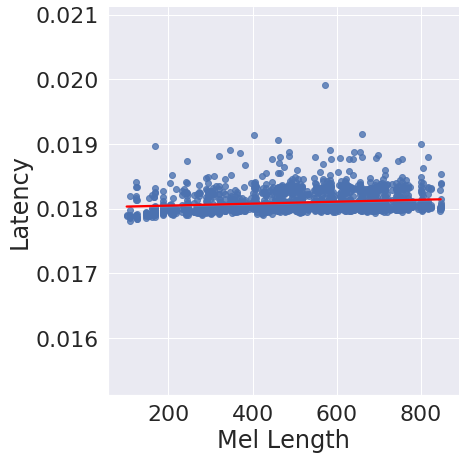
\includegraphics[width=0.6\textwidth]{images/len-lat.png}
\caption{Non-autoregressive and attention-less pipeline effect}
\end{figure}
\end{frame}

\begin{frame}{Results}
\begin{itemize}
    \item $320$x realtime generations speed
    \item 10M weights: 3x times less than competitors.
    \item New 2-stage pipeline
    \item ASR as a teacher model instead of TTS
    \item Attention-less architecture
    \item Paper~\footcite{beliaev2020talknet}
\end{itemize}
\end{frame}

\begin{frame}{Литература}
\printbibliography[heading=none]
\end{frame}

\end{document}